\documentclass[handout]{beamer}\mode<presentation>{\usetheme{AMSCesenaBleu}}
% \documentclass[presentation]{beamer}\mode<presentation>{\usetheme{AMSCesenaBleu}}
%%%%

\usepackage{common}
\usepackage{courses}

\title[L8 -- Process algebrae]{Process algebrae fundamentals}
%
\subtitle[SD]
{Distributed Systems / Technologies\\\scriptsize Sistemi Distribuiti / Tecnologie}
%
\author[Ciatto \and Omicini]
{\alert{Giovanni Ciatto} \and \emph{Andrea Omicini}\\
\texttt{giovanni.ciatto@unibo.it \and andrea.omicini@unibo.it}}
%
\institute[DISI, Univ. Bologna]
{Dipartimento di Informatica -- Scienza e Ingegneria (DISI)\\\textsc{Alma Mater Studiorum} -- Universit{\`a} di Bologna a Cesena}
%
\date[A.Y. 2019/2020]{Academic Year 2019/2020}

\setbeamercovered{transparent}

\begin{document}

\maketitle

\begin{frame}[c]\frametitle{Outline}
    \begin{multicols}{2}
	    \tableofcontents[sectionstyle=show/show, subsectionstyle=show/show, subsubsectionstyle=show/show]
    \end{multicols}
\end{frame}

\section{Lecture goals} 

\begin{frame}%[allowframebreaks]
    \frametitle{Lecture goals I}

    \begin{itemize}
        \item<1> Designing and implementing concurrent/distributed system (C/DS) is hard also because it is difficult to 
        %
        \begin{itemize}
            \item<1> precisely specify the behaviour of a C/DS
            \item<1> verify a protocol correctly works in \alert{all possible situations}
        \end{itemize}
        
        \vfill
        
        \item<2> Here we will exemplify how process algebra-based modelling and reasoning may ease both a C/DS \alert{specification} -- making it clearer and more precise --, and its \alert{verification}---enabling us to prove some properties always hold (e.g. termination, deadlock-freedom, etc.)
        
        \vfill
        
        \item<3> Computer scientists are usually interested in proving general the \alert{correctness} of a C/DS
        %
        \begin{itemize}
            \item<3>[e.g.] the PayPal payment protocol MUST be deadlock-free, and MUST guarantee a 0-or-1 semantics to payments, in ANY possibile scenario
        \end{itemize}
        
        \vfill
        
        \item<4> Software engineers are usually interested in precisely specifing the \alert{semantics} of the software they are designing
        %
        \begin{itemize}
            \item<4>[e.g.] what do you exactly mean by ``the \texttt{in} operation must suspend in case no tuple is available?''
        \end{itemize}
        
    \end{itemize}
    
\end{frame}

\begin{frame}%[allowframebreaks]
    \frametitle{\linda{} as a running example}

    \begin{itemize}
        \item<1> In giving you the \linda{} specification during the previous Lab lessons, we deliberately used the natural language, often issuing \alert{ambiguous} statements on purpose
        
        \vfill
        
        \item<2> The aim was to let you understand that several arbitrary \alert{interpretations} may be derived from an ambiguous specification
        %
        \begin{itemize}
            \item<2> which is a nightmare for engineers
        \end{itemize}
        
        \vfill
        
        \item<3> You should already have implemented \linda{}. We will now \alert{model} (i.e. design) it by means of CCS, transition rules, and labelled transition systems
        
        \vfill
        
        \item<4> We will then show how several semantics could be defined from the same natural language-based specification 
    \end{itemize}
    
\end{frame}

\section{Syntax and Semantics}

\begin{frame}
\frametitle{A workflow for semantics specification}
    
    In order to \alert{formally} model a C/DS using the \href{https://en.wikipedia.org/wiki/Calculus_of_communicating_systems}{Calculus of Communicating Systems} (CCS), and define its semantics, one usually need to perform the following steps:
    %
    \begin{enumerate}
        \item<1> Define a \alert{syntax} for the C/DS system, covering all possible situations
        %
        \begin{itemize}
            \item<1> this can be done by means of \alert{grammars}, which is employed to define operators, actions, and processes
        \end{itemize}
        
        \item<2> Instantiate a particular C/DS system as a \alert{word} over the language generated by the grammar above
        
        \item<3> Define its semantics in terms of a \alert{Labelled Transition System} (LST), which usually implies:
        %
        \begin{itemize}
            \item<3> formalise the \alert{transition rules} governing the system behaviour
            \item<3> adopting the aforementioned word as the \alert{initial state}
            
            \item<3> generating the graph of possible states for the system by recursively applying all enabled transition rules to the initial state
        \end{itemize}
        
        \item<4> Verify properties over the LTS by means of \alert{model-checkers} and \alert{temporal logics} (we won't do that) 
    \end{enumerate}
    
\end{frame}


\section{Formalising \linda{}}

\begin{frame}
\frametitle{Formalising \linda{} with process algebrae}

    We will now provide an example showing how process algebrae could be employed to formally describe the semantics of \linda{}
    %
    \vfill
    %
    \begin{enumerate}
        \item<1> We will model tuple spaces by means of CCS
        
        \vfill
        
        \item<2> We will then provide their formal semantics as standalone systems, by means of a LTS
        
        \vfill
        
        \item<3> We will model agents/users by means of CCS
        
        \vfill
        
        \item<4> We will then provide their formal semantics as standalone systems, by means of a LTS
        
        \vfill
        
        \item<5> Finally we will provide the syntax and the semantics of a \alert{coordinated system}, i.e., the \alert{parallel composition} of several agents/users interacting with and by means of a tuple space
    \end{enumerate}
\end{frame}

\subsection{Tuple Spaces}

\subsubsection{Syntax}

\begin{frame}
\frametitle{Tuple Spaces -- Syntax}

    \begin{block}{A grammar for \linda{'s} tuple space processes}
        \[\begin{array}{rcll}
            TS &::=& (T \cup TS) \mid (\langle T \rangle \cup TS) \mid \emptyset & \mathhint{tuple spaces}\\
            \\
            T &::=& t \mid t' \mid t'' \mid \cdots \mid t_1 \mid t'_1 \mid t''_1 \mid \cdots & \mathhint{tuples}
        \end{array}\]
    \end{block}
    
    \hint{$\langle t \rangle$ represents a tuple that is going to be inserted within the tuple space}
    
    \pause\vfill
    
    \begin{block}{Subject to the following axioms}
        \[\begin{array}{rcll}
            X \cup Y &\equiv& Y \cup X & \mathhint{union is commutative} \\
            X \cup (Y \cup Z) &\equiv& (X \cup Y) \cup Z & \mathhint{parentheses are useless for unions}\\
            X \cup \emptyset &\equiv& X & \mathhint{neutral element for union}
        \end{array}\]
    \end{block}
\end{frame}

\begin{frame}
\frametitle{Tuple Spaces -- Several possible processes}
    
    Several tuple space processes could be syntactically represented by means of this grammar:
    %
    \vfill{}
    %
    \begin{itemize}
        \item<1>[e.g.] $ts_0 = \emptyset$
        
        \vfill
        
        \item<2>[e.g.] $ts_1 = t {\ \color{gray}\equiv t \cup \emptyset \equiv \emptyset \cup t \equiv t \cup \emptyset \cup \emptyset }$
        
        \vfill
        
        \item<3>[e.g.] $ts_2 = t_1 \cup t_2 {\ \color{gray} \equiv t_1 \cup t_2 \cup \emptyset \equiv t_2 \cup t_1 \equiv t_1 \cup \emptyset \cup t_2 }$
        
        \vfill
        
        \item<4>[e.g.] $ts_3 = t_1 \cup t_2 \cup t_3 {\ \color{gray} \equiv t_1 \cup t_2 \cup t_3 \cup \emptyset }$
        
        \vfill
        
        \item<5>[e.g.] $ts_3 = t_1 \cup \langle t_2 \rangle \cup t_3 \cup \langle t_2 \rangle$
        
    \end{itemize}
    
    \vfill
    
    \begin{block}{}
        We say that $ts_0$, $ts_1$, $ts_2$, $ts_3$ are \alert{words} in $\mathcal{L}(TS)$, namely, the language generated by $TS$, i.e., the set of all possible tuples
        %
        % Oftern, for covenience, we simply write 
    \end{block}
    
\end{frame}

\subsubsection{Semantics}

\begin{frame}
\frametitle{Tuple Spaces -- Semantics}

    \begin{block}{A grammar for tuple space related \textbf{events}}
        \[\begin{array}{rcll}
            E_{TS} &::=& !O_{TS} \mid ?I_{TS}  \mid \tau & \mathhint{event for tuple spaces} \\
            O_{TS} &::=& in(T) \mid rd(T) & \mathhint{output events} \\
            I_{TS} &::=& out(T) & \mathhint{input events} \\
        \end{array}\]
    \end{block}
    
    \pause

    \begin{block}{\linda{'s} tuple spaces as a Labelled Transition System}
        We define a tuple space $\mathcal{TS}$ as a LTS, i.e. a \emph{quartet} $ \langle S,\, s_0,\, \longrightarrow_\mathcal{TS},\, E \rangle$ where:
        %
        \begin{itemize}
            \item $S = \mathcal{L}(TS)$ is a set of possible \alert{states}
            \item $s_0 \in S$ is the \alert{initial} state
            \item $E = \mathcal{L}(E_{TS})$ is a set of event \alert{labels}
            \item $\longrightarrow_\mathcal{TS}\ \subseteq (S \times E \times S)$ is the set of admissible \alert{transitions}
        \end{itemize}
        % \[\begin{array}{rcl}
        %     TS &::=& (T \cup TS) \mid \emptyset\\
        %     T &::=& t \mid t' \mid t'' \mid \cdots \mid t_1 \mid t'_1 \mid t''_1 \mid \cdots
        % \end{array}\]
    \end{block}
    
    % \begin{block}{Subject to the following axioms}
    %     \[\begin{array}{rcll}
    %         X \cup Y &\equiv& Y \cup X & \mathhint{union is commutative} \\
    %         X \cup (Y \cup Z) &\equiv& (X \cup Y) \cup Z & \mathhint{parentheses are useless for unions}\\
    %         X \cup \emptyset &\equiv& X & \mathhint{neutral element for union}
    %     \end{array}\]
    % \end{block}
\end{frame}

\subsubsection{Transition Rules}

\begin{frame}
\frametitle{Transition Rules}

    \begin{block}{}
        The set of admissible transitions $\longrightarrow_\mathcal{TS}$ is usually \alert{intensionally} defined by means of transition rules matching the following pattern:
        %
        \[
            \frac{C_1,\ \ldots,\ C_N}{s \stackrel{e}{\longrightarrow}_\mathcal{TS} s'} \qquad [\text{RULE-NAME}]
        \]
        %
        meaning that transition $(s, e, s') \in \longrightarrow_\mathcal{TS}$ only if \alert{preconditions} $C_1$, \ldots, $C_n$ hold within the source state $s$
    \end{block}
    %
    \pause
    %
    \begin{itemize}
        \item If no precondition of interest need to be specified, the numerator and the fraction line are usually omitted
        
        \pause
        
        \item The states $s$ and $s'$ are usually represented by means of non-ground formulas containing both terminal and non-terminal symbols, i.e. variables
        %
        \begin{itemize}
            \item you can then imagine a transition rule as a \alert{rewriting rule}
        \end{itemize}
    \end{itemize}

\end{frame}

\begin{frame}
\frametitle{Tuple Spaces  -- Transition Rules}
    So, for what concerns \linda{} tuple spaces, we define the following transition rules:
    
    \[\begin{array}{rclr}
        \onslide<1>{TS &\xrightarrow{?out(t)}_\mathcal{TS}& TS \cup \langle t \rangle & [\text{SCHEDULE}]} \\
        \\
        \onslide<2>{TS \cup \langle t \rangle &\xrightarrow{\phantom{ab}\tau\phantom{ab}}_\mathcal{TS}& TS \cup t & [\text{INSERT}]} \\
        \\
        \onslide<3>{TS \cup t &\xrightarrow{!in(t)}_\mathcal{TS}& TS & [\text{CONSUME}]} \\
        \\
        \onslide<4>{TS \cup t &\xrightarrow{!rd(t)}_\mathcal{TS}& TS \cup t & [\text{OBSERVE}]} \\
    \end{array}\]
    
\end{frame}

\begin{frame}
\frametitle{Tuple Spaces  -- The state graph}
    
    \begin{columns}
        \begin{column}{.75\linewidth}
            \begin{exampleblock}{Example where $s_0 = \emptyset$}
                \href{http://www.plantuml.com/plantuml/svg/RP1FJi905CRtSuhd2ZKXAGKs3K52mMYYa5XnWomczAaJfZFDp6iKZJjDN70HkOntu2IEJ6fgxAvvl-_FrnbOueQAJ3Ax4YhdXcSmmZjUI3hLYXBnZ1065PWG9zmZMai4GLoAfQrtJtY64El223JiGQG8cEMqXXJjqeYSX5QiuhG_qV3208PykRetkb1fhAKslTvCuLFklZ3jzs6DKkf7zihO_7W1pMOVRC2ysGOHx3xUcGtylHN1YIxea8vkrJo9pyQZsSLuKOeTtMq-QRVPCjloXZ22hpUdFPyauwlhNwKx4xEXrxYE0w5yPZoT9BDB5rd2q46JUZWTkf2R2coNSngrUnmcDt-xNzNOpsfxOwUkieJjkieITkj_g0D_7pMgT7f5zv_2RwC66w1AYqn-0m00}{http://www.plantuml.com/plantuml/svg/RP1...0m00}
            \end{exampleblock}
            
            \vfill
            
            \[\begin{array}{rclr}
                TS &\xrightarrow{?out(t)}_\mathcal{TS}& TS \cup \langle t \rangle & [\text{SCHEDULE}] \\
                \\
                TS \cup \langle t \rangle &\xrightarrow{\phantom{ab}\tau\phantom{ab}}_\mathcal{TS}& TS \cup t & [\text{INSERT}] \\
                \\
                TS \cup t &\xrightarrow{!in(t)}_\mathcal{TS}& TS & [\text{CONSUME}] \\
                \\
                TS \cup t &\xrightarrow{!rd(t)}_\mathcal{TS}& TS \cup t & [\text{OBSERVE}] \\
            \end{array}\]
        \end{column}
        \begin{column}{.25\linewidth}
            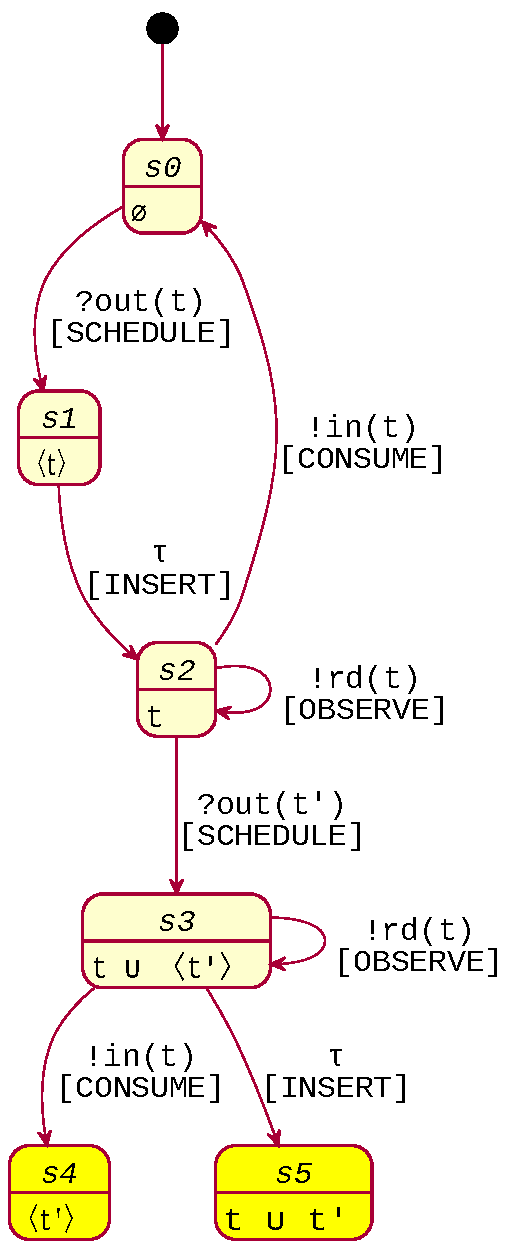
\includegraphics[width=\linewidth]{res/img/ts_lts.pdf}
        \end{column}
    \end{columns}
    
\end{frame}

\subsection{Users}

\subsubsection{Syntax}

\begin{frame}
\frametitle{Users -- Syntax}

    \begin{block}{A grammar for User processes}
        \[\begin{array}{rcll}
            U &::=& \mathtt{out}(T) \cdot U \mid \mathtt{in}(TT) \cdot U \mid \mathtt{rd}(TT) \cdot U & \mathhint{users} \\
            &\mid& \langle T \rangle \mid (U + U) \mid 0\\
            \\
            TT &::=& \bar{t} \mid \bar{t}' \mid \bar{t}'' \mid \cdots \mid \bar{t}_1 \mid \bar{t}'_1 \mid \bar{t}''_1 \mid \cdots & \mathhint{templates}
        \end{array}\]
    \end{block}
    %
    \hint{where $\langle t \rangle$ represent the result of an access action}
    %
    \pause\vfill
    %
    \begin{block}{Subject to the following axioms}
        \vspace{-.4cm}
        \[\begin{array}{rcll}
            X \cdot Y &\not\equiv& Y \cdot X & \mathhint{sequence is non-commutative}\\
            X \cdot (Y \cdot Z) &\equiv& (X \cdot Y) \cdot Z & \mathhint{parentheses are useless for sequences}\\
            X \cdot 0 &\equiv& X & \mathhint{neutral element for sequences}\\
            \hline
            X + Y &\equiv& Y + X & \mathhint{choice is commutative}\\
            X + (Y + Z) &\equiv& (X + Y) + Z & \mathhint{parentheses are useless for choices}\\
            % X \cdot X &\equiv& X & \mathhint{neutral element for choices}\\
            (X + Y) \cdot Z &\equiv& X \cdot Z + Y \cdot Z & \mathhint{choice is right-distributive w.r.t sequence}\\
        \end{array}\]
    \end{block}
\end{frame}

\begin{frame}
\frametitle{Users -- Several possible processes}
    
    Several user processes could be syntactically represented by means of this grammar (not always making sense):
    %
    \vfill{}
    %
    \begin{itemize}
        \item<1>[e.g.] $u_0 = \mathtt{in}(\bar t) \cdot \langle t \rangle \cdot \mathtt{out}(t') \cdot \mathtt{rd}(\bar{t}'') \cdot \langle t'' \rangle \cdot 0$
        \vfill
        \item<2>[e.g.] $u_1 = \mathtt{out}(t_1) \cdot \mathtt{out}(t_2) \cdot \mathtt{out}(t_3) \cdot \mathtt{rd}(\bar t) \cdot \langle t \rangle \cdot 0$
        \vfill
        \item<3>[e.g.] $u_2 = (\mathtt{in}(\bar{t}_1) + \mathtt{in}(\bar{t}_2) + \mathtt{in}(\bar{t}_3)) \cdot \langle t \rangle \cdot 0$
        \vfill
        \item<4>[e.g.] $u_3 = \langle t \rangle \cdot \mathtt{in}(\bar{t}) \cdot \langle t' \rangle \cdot \mathtt{rd}(\bar{t}') \cdot 0$ \hint{makes no sense}
        \vfill
        \item<5>[e.g.] $u_4 = \mathtt{in}(\bar{t}) \cdot \langle t \rangle \cdot \mathtt{out}(t') \cdot u_4$ \hint{recursive}
        
    \end{itemize}
    
\end{frame}

\subsubsection{Semantics}

\begin{frame}
\frametitle{Users -- Semantics}

    \begin{block}{A grammar for tuple space related \textbf{events}}
        \[\begin{array}{rcll}
            E_{U} &::=& !O_U \mid ?I_U  \mid \tau & \mathhint{events for users} \\
            O_U &::=& out(T) & \mathhint{output events} \\
            I_U &::=& rd(TT) \mid in(TT)  & \mathhint{input events} \\
        \end{array}\]
    \end{block}
    
    \pause

    \begin{block}{\linda{'s} users as a Labelled Transition System}
        We define a user $\mathcal{U}$ as a LTS, i.e. a \emph{quartet} $ \langle S,\, s_0,\, \longrightarrow_\mathcal{U},\, E \rangle$ where:
        %
        \begin{itemize}
            \item $S = \mathcal{L}(U)$ is a set of possible \alert{states}
            \item $s_0 \in S$ is the \alert{initial} state
            \item $E = \mathcal{L}(E_{U})$ is a set of event \alert{labels}
            \item $\longrightarrow_\mathcal{U}\ \subseteq (S \times E \times S)$ is the set of admissible \alert{transitions}
        \end{itemize}
    \end{block}
\end{frame}

\subsubsection{Transition Rules}

\begin{frame}
\frametitle{Users  -- Transition Rules}
    For what concerns \linda{} users, we define the following transition rules:
    
    \[\begin{array}{rclr}
        \onslide<1>{\mathtt{out}(t) \cdot U &\xrightarrow{!out(t)}_\mathcal{U}& U & [\text{WRITE}]} \\
        \\
        \onslide<2>{\mathtt{rd}(\bar t) \cdot U &\xrightarrow{?rd(\bar t)}_\mathcal{U}& U & [\text{READ}]} \\
        \\
        \onslide<3>{\mathtt{in}(\bar t) \cdot U &\xrightarrow{?in(\bar t)}_\mathcal{U}& U & [\text{TAKE}]} \\
        \\
        \onslide<4>{\langle t \rangle \cdot U &\xrightarrow{\phantom{ab}\tau\phantom{ab}}_\mathcal{U}& U & [\text{COMPUTE}]}
    \end{array}\]
    %
    \onslide<5>$
        \frac{U_1 \cdot U'_1 \xrightarrow{\phantom{ab}E\phantom{ab}}_\mathcal{U} U'_1}{U_1 \cdot U'_1 + U_2 \cdot U'_2 \xrightarrow{\phantom{ab}E\phantom{ab}}_\mathcal{U} U'_1} \quad [\text{CHOICE-L}]
    $ 
    \hfill
    \onslide<6>$
        \frac{U_2 \cdot U'_2 \xrightarrow{\phantom{ab}E\phantom{ab}}_\mathcal{U} U'_2}{U_1 \cdot U'_1 + U_2 \cdot U'_2 \xrightarrow{\phantom{ab}E\phantom{ab}}_\mathcal{U} U'_2} \quad [\text{CHOICE-R}]
    $ 
    
    \vfill
    
    \begin{block}{}
        Notice that no rule exists matching state $0$ since it represents termination
    \end{block}
    
\end{frame}

\begin{frame}
\frametitle{Users -- The state graph}
    
    Example where \alert{$s_0 = \mathtt{out}(t_1) \cdot (\mathtt{rd}(\bar{t}_2) + \mathtt{in}(\bar{t}_2)) \cdot \langle t_2 \rangle \cdot \mathtt{in}(\bar{t}_3) \cdot \mathtt{rd}(\bar{t}_1) \cdot 0$}

    \begin{columns}
        \begin{column}{.70\linewidth}
            \small
            \[\begin{array}{rclr}
                \mathtt{out}(t) \cdot U &\xrightarrow{!out(t)}_\mathcal{U}& U & [\text{WRITE}] \\
                \\
                \mathtt{rd}(\bar t) \cdot U &\xrightarrow{?rd(\bar t)}_\mathcal{U}& U & [\text{READ}] \\
                \\
                \mathtt{in}(\bar t) \cdot U &\xrightarrow{?in(\bar t)}_\mathcal{U}& U & [\text{TAKE}] \\
                \\
                \langle t \rangle \cdot U &\xrightarrow{\phantom{ab}\tau\phantom{ab}}_\mathcal{U}& U & [\text{COMPUTE}]
            \end{array}\]
            %
            \[
                \frac{U_1 \cdot U'_1 \xrightarrow{\phantom{ab}E\phantom{ab}}_\mathcal{U} U'_1}{U_1 \cdot U'_1 + U_2 \cdot U'_2 \xrightarrow{\phantom{ab}E\phantom{ab}}_\mathcal{U} U'_1} \quad [\text{CHOICE-L}]
            \]
            %
            \[
                \frac{U_2 \cdot U'_2 \xrightarrow{\phantom{ab}E\phantom{ab}}_\mathcal{U} U'_2}{U_1 \cdot U'_1 + U_2 \cdot U'_2 \xrightarrow{\phantom{ab}E\phantom{ab}}_\mathcal{U} U'_2} \quad [\text{CHOICE-R}]
            \]
        \end{column}
        \begin{column}{.30\linewidth}
            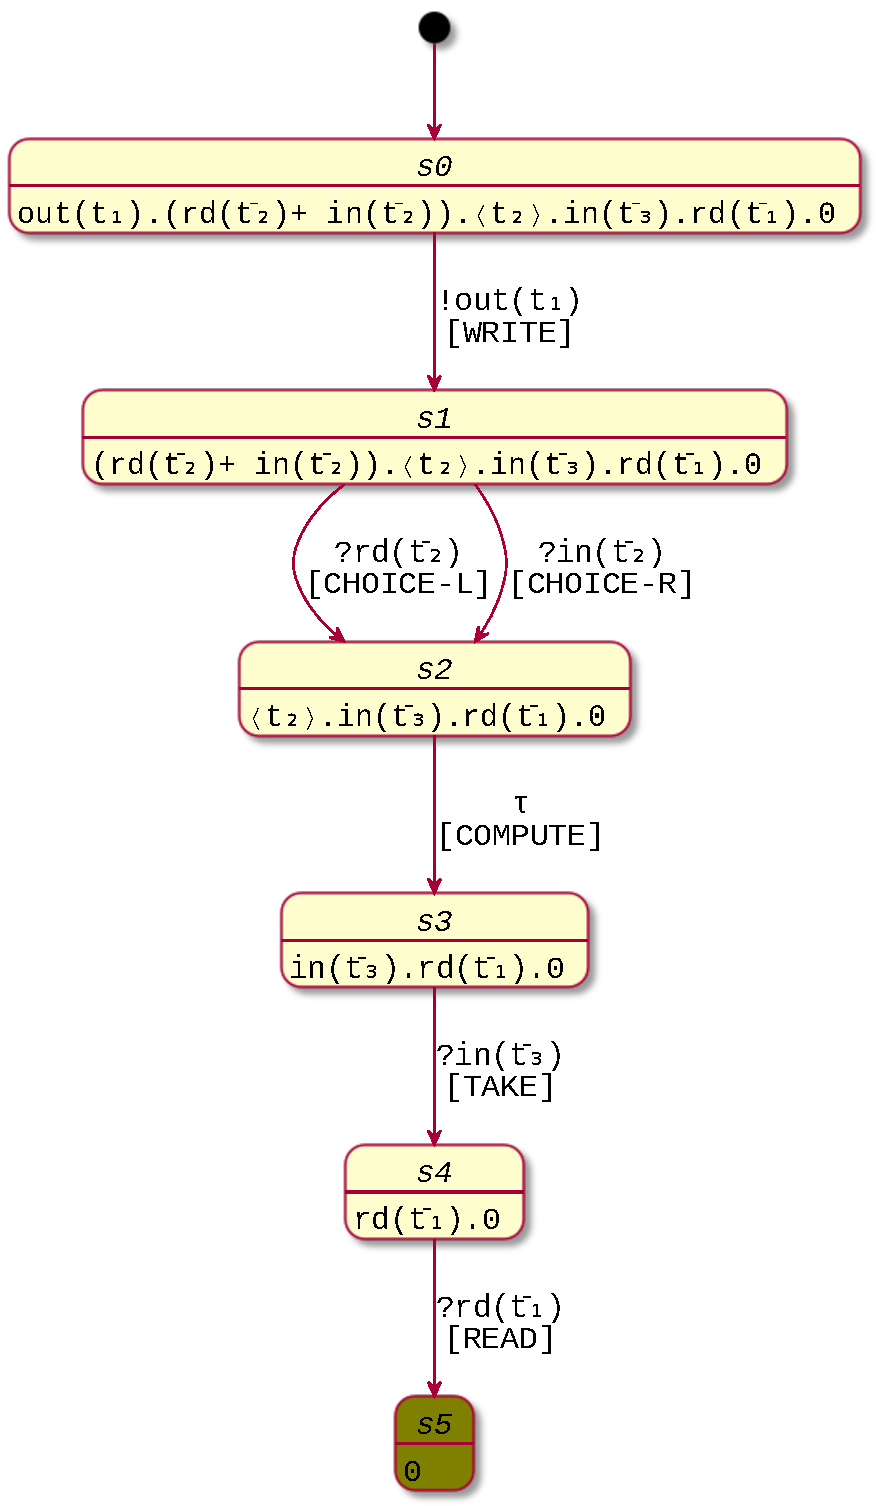
\includegraphics[width=\linewidth]{res/img/user.pdf}
            
            \hint{Zoomable image \href{http://www.plantuml.com/plantuml/svg/fPBDJl9058RtSnNdsz7Fq9G2cuOWM6ea_c3uYGjaCQ4ZJfZEDDEfYiQ5m98RqMinyHvw9GusjIN1nCJTIUTzdlTCCwr8OQdYWA5eJdc89GwWGsvmpDInu6f07mdOLk5meB0YNqTgmGXGXHcTHllf2nmGS4KiAP7eble4I12g1VWacaeQAYeuAf3HLWrF2E08J-SpAMBkku89sMXutATyrco2OFIEx4kCE7a8zKHydLeGniGzUaPe_7y2vN8J8Wkb-iXoGCIgf9BbYs6Mf5zIx-jakJGEWF9iDinaywhqb6pUpEppoZ2pj2QrpqhD5GV-VHkl-VYgtnrw4vJrLS21FzLKqXhRWSDSetlSarxNzSfdavr8RiyZ_NmR6npuJQcT6giEVAotejxvvQXugwhs_0XNKxXMM6UrNMVOFYqeQbgnozLIhfxVDFsZVQ_ToRawvE_10GkX5k5-7B1F}{here}}
        \end{column}
    \end{columns}
    
\end{frame}

\subsection{Coordinated Systems}

\subsubsection{Syntax}

\begin{frame}
\frametitle{Coordinated Systems -- Syntax}

    \begin{block}{A grammar for coordinated systems}
        \[\begin{array}{rcll}
            CS &::=& US \parallel TS & \mathhint{coordinated system}\\
            US &::=& (U \parallel US) \mid 0 & \mathhint{list of users}
        \end{array}\]
    \end{block}
    
    \pause
    
    \begin{block}{Subject to the following axioms}
        \[\begin{array}{rcll}
            X \parallel Y &\not\equiv& Y \parallel X & \mathhint{parallel is \alert{not} commutative} \\
            X \parallel (Y \parallel Z) &\equiv& (X \parallel  Y) \parallel Z & \mathhint{parentheses are useless for unions} \\
            X \parallel 0 &\equiv& X & \mathhint{neutral element for parallel}
        \end{array}\]
    \end{block}
    %
    \hint{A non-commutative parallel operator makes the processes identifiable by means of their \emph{index}}
    
    \pause\vfill
    
    \begin{block}{}
	    Notice that the states of a coordinated systems must match the patterns:
	    %
	    \[\begin{array}{c}
	        U_1 \parallel \cdots \parallel U_i \parallel \cdots \parallel U_n \parallel TS\\
	        US \parallel U_i \parallel US' \parallel TS
	 	\end{array}\]
    \end{block}
    
\end{frame}

\subsubsection{Semantics}

\begin{frame}
\frametitle{Coordinated Systems -- Semantics}

    \begin{block}{A grammar for coordinated systems related \textbf{events}}
        \[\begin{array}{rcll}
            E_{CS} &::=& out(T) \mid in(T) \mid rd(T) \mid \tau & \mathhint{events} \\
        \end{array}\]
    \end{block}
    
    \pause

    \begin{block}{Coordinated systems as a Labelled Transition System}
        We define a user $\mathcal{CS}$ as a LTS, i.e. a \emph{quartet} $ \langle S,\, s_0,\, \longrightarrow_\mathcal{CS},\, E \rangle$ where:
        %
        \begin{itemize}
            \item $S = \mathcal{L}(CS)$ is a set of possible \alert{states}
            \item $s_0 \in S$ is the \alert{initial} state
            \item $E = \mathcal{L}(E_{CS})$ is a set of event \alert{labels}
            \item $\longrightarrow_\mathcal{CS}\ \subseteq (S \times E \times S)$ is the set of admissible \alert{transitions}
        \end{itemize}
    \end{block}
\end{frame}

\subsubsection{Transition Rules}

\begin{frame}
\frametitle{Coordinated Systems -- Transition Rules I}

    For what concerns coordinated systems, we define the following transition rules (pay attention to the \alert{indexes} in rules names):
    
    \onslide<1>\[
        \frac{
            \mathtt{out}(t) \cdot U_i \xrightarrow{\highlightG{!out(t)}}_\mathcal{U} U_i 
            \qquad
            TS \xrightarrow{\highlightG{?out(t)}}_\mathcal{TS} TS \cup \langle t \rangle 
        }{
            US \parallel \highlightR{\mathtt{out}(t) \cdot U_i} \parallel US' \parallel \highlightB{TS}
            \xrightarrow{\highlightG{out(t)}}_\mathcal{CS}
            US \parallel \highlightR{U_i} \parallel US' \parallel \highlightB{TS \cup \langle t \rangle}
        } 
        \quad 
        [\text{OUT}_i]
    \]
    
    \onslide<2>\[
		\frac{
			\mathtt{in}(\bar t) \cdot U_i \xrightarrow{\highlightG{?in(\bar t)}}_\mathcal{U} U_i 
			\qquad
			TS \cup t \xrightarrow{\highlightG{!in(t)}}_\mathcal{TS} TS
			\qquad
			t \in \bar{t}
		}{
			US \parallel \highlightR{\mathtt{in}(\bar t) \cdot U_i} \parallel US' \parallel \highlightB{TS \cup t}
			\xrightarrow{\highlightG{in(t)}}_\mathcal{CS}
			US \parallel \highlightR{\langle t \rangle \cdot U_i} \parallel US' \parallel \highlightB{TS}
		} 
		\quad 
		[\text{IN}_i]
	\]
	
	\onslide<3>\[
		\frac{
			\mathtt{rd}(\bar t) \cdot U_i \xrightarrow{\highlightG{?rd(\bar t)}}_\mathcal{U} U_i 
			\qquad
			TS \cup t \xrightarrow{\highlightG{!rd(t)}}_\mathcal{TS} TS \cup t
			\qquad
			t \in \bar{t}
		}{
			US \parallel \highlightR{\mathtt{rd}(\bar t) \cdot U_i} \parallel US' \parallel \highlightB{TS \cup t}
			\xrightarrow{\highlightG{rd(t)}}_\mathcal{CS}
			US \parallel \highlightR{\langle t \rangle \cdot U_i} \parallel US' \parallel \highlightB{TS \cup t}
		} 
		\quad 
		[\text{RD}_i]
	\]

\end{frame}

\begin{frame}
\frametitle{Coordinated Systems -- Transition Rules II}
	%
	\onslide<1>\[
		\frac{
			\langle t \rangle \cdot U_i \xrightarrow{\highlightG{\phantom{ab}\tau\phantom{ab}}}_\mathcal{U} U_i 
		}{
			US \parallel \highlightR{\langle t \rangle \cdot U_i} \parallel US' \parallel TS
			\xrightarrow{\highlightG{\phantom{ab}\tau\phantom{ab}}}_\mathcal{CS}
			US \parallel \highlightR{U_i} \parallel US' \parallel TS
		} 
		\quad 
		[\text{COMPUTE}_i]
	\]
	
	\onslide<2>\[
		\frac{
			TS \cup \langle t \rangle \xrightarrow{\highlightG{\phantom{ab}\tau\phantom{ab}}}_\mathcal{TS} TS \cup t
		}{
			US \parallel \highlightB{TS \cup \langle t \rangle}
			\xrightarrow{\highlightG{\phantom{ab}\tau\phantom{ab}}}_\mathcal{CS}
			US \parallel \highlightB{TS \cup t}
		} 
		\quad 
		[\text{INSERT}]
	\]
	
	\onslide<3-4>\[
		\frac{
			U_i + U'_i \xrightarrow{\highlightG{\phantom{ab}E'\phantom{ab}}}_\mathcal{U} U''_i 
			\qquad
			TS \xrightarrow{\highlightG{\phantom{ab}E''\phantom{ab}}}_\mathcal{TS} TS'
			\qquad
			E = \gamma(E', E'')
		}{
			US \parallel \highlightR{U_i + U'_i} \parallel US' \parallel \highlightB{TS}
			\xrightarrow{\highlightG{\phantom{ab}E\phantom{ab}}}_\mathcal{CS}
			US \parallel \highlightR{U''_i} \parallel US' \parallel \highlightB{TS'}
		} 
		\quad 
		[\text{CHOICE}_i]
	\]
	%
	\onslide<4>{
		where the partial funtion $\gamma(\cdot, \cdot)$ is defined as follows:
		%
        \begin{multicols}{2}\begin{itemize}
            \item $\gamma(!out(t), ?out(t)) = out(t)$
		    \item $\gamma(?in(\bar t), !in(t)) = in(t)$
		    \item $\gamma(?rd(\bar t), !rd(t)) = rd(t)$
        \end{itemize}\end{multicols}
        % }
	}
\end{frame}

\begin{frame}
\frametitle{Example: Out-In-Rd, \emph{unordered}}
    Example where \alert{$s_0 = \mathtt{out}(t) \cdot 0 \parallel \mathtt{in}(\bar t) \cdot 0 \parallel \mathtt{rd}(t) \cdot 0 \parallel \emptyset$}
    
    \begin{center}
        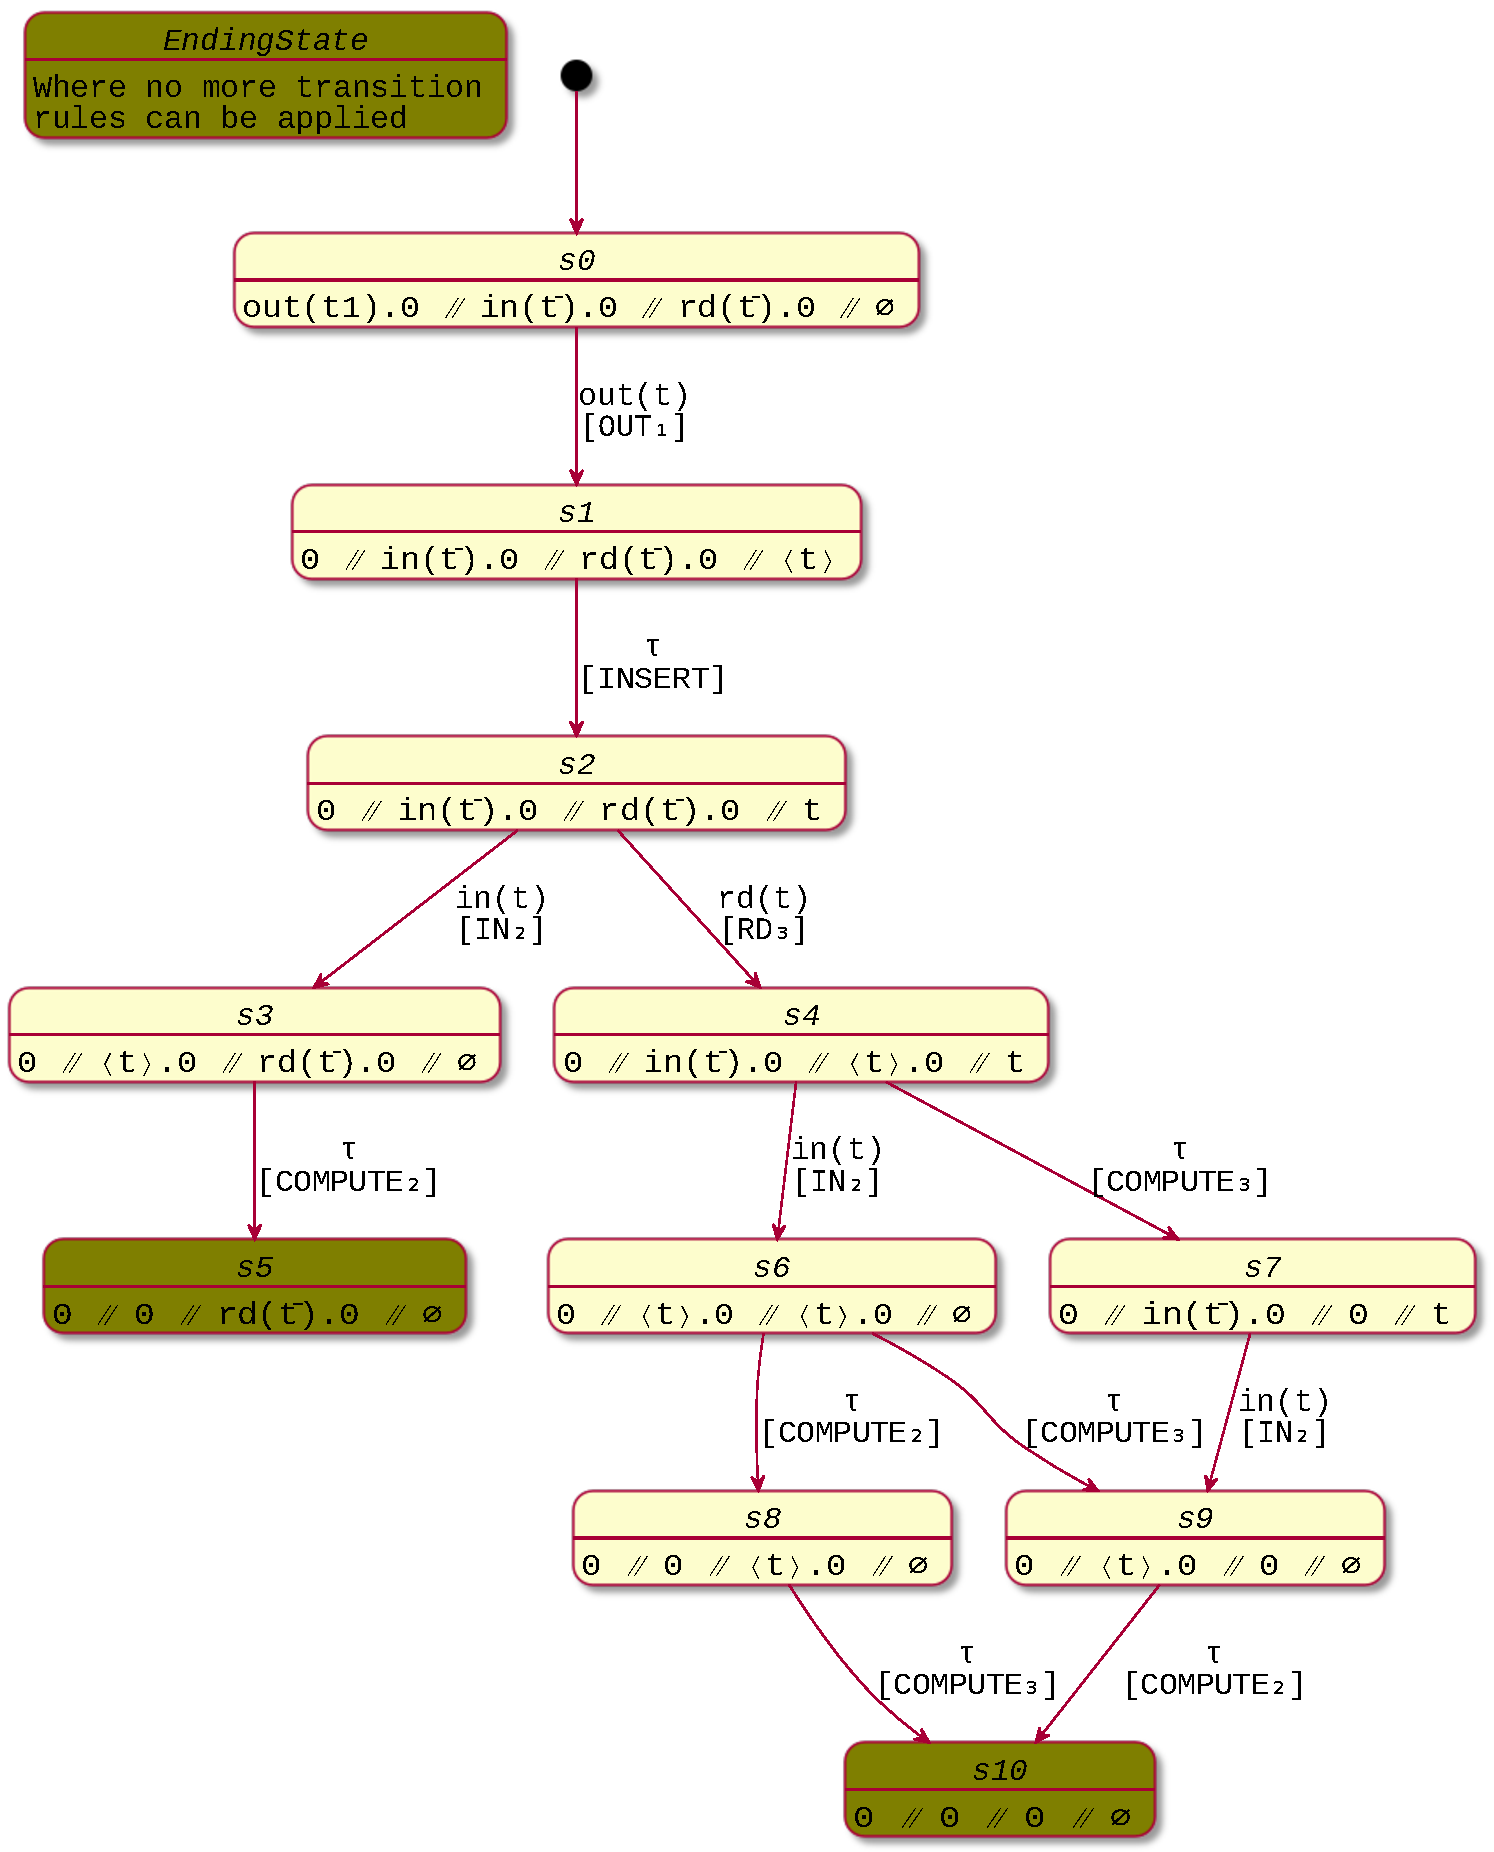
\includegraphics[width=.4\linewidth]{res/img/out_in_rd.pdf}
        
        \hint{Zoomable image \href{http://www.plantuml.com/plantuml/svg/ZP9FRXCn5CRtFiLRDaX5apJDdr4LLQH1Oa6BcbGisYnCvj5QzTWZ-mrIGIm8HMBHQx20io1nXpa9apYEfz5CrKKMpkVtUx_FccDBt52UIcPlXSguuIcSu4UUItgj5Kt5PuHEL0cdn0dN4Tr9145SYeMjdpxbAS9OvqQWOJSYGS0qepj8q2wCo4XenIgJTeM6BmpW5L_SNXkTgsIifJP7HnEL27Kz6e6MuXEohuovo-x_jHE4Mp6ylq63e3IasY2GuSgArRehPNA95XPSmGS4dcLIOCBOvOivxE-Fm4ORi8rYq3djKRlrCeBYvoyGQe_-tlkJIIgdylU3sSWHsfl1rfMwFBkO5SjlSs-xofu1U_XDnSCVPjiEs8dXttq9UtCwdPpF0gpp71Wnst6OWtXziRKc5SlbV9jqutB89USdnV9xM57EF79gBd_WK8SRr_7PstSNiqcv9i2wjRu1xNsx3jNRzTqc_Tqb5UF3Hv-1OpP9-vbURSjm2YrxJc1Gqz9dmoVa-lKli6tUzuZTvXumy816mu53jACdD8RrVIkKOHCbk9HXurC7qZ6g94_bVm00}{here}}
    \end{center}
\end{frame}

\subsection{Exercise 5-1}

\begin{frame}
\frametitle{Exercise 5-1: Out-Out-In-In, \emph{unordered} I}
    \begin{enumerate}
        \item Clone the Lab-5 GitLab repository: \url{https://gitlab.com/pika-lab/courses/ds/aa1819/lab-5}
        
        \vfill
        
        \item Consider the system with \alert{$s_0 = \mathtt{out}(t_1) \cdot \mathtt{out}(t_2) \cdot \mathtt{in}(\bar t) \cdot \mathtt{in}(\bar t) \cdot 0  \parallel \emptyset$}, where $t_1, t_2 \in \bar{t}$, s.t. the \linda{} semantics defined before
        
        \vfill
    
        \item Complete the state graph according to the transition ruled defined before and include the state graph image in your \alert{\texttt{README.md}} file
        %
        \begin{itemize}
            \item web editor here: \href{
                http://www.plantuml.com/plantuml/uml/ZPBVJl8m6CRFUnNl8Nm9P8m_4488-H0JJp0HE48E6bQneMkNjLFHUE22YGVSXWToBIRU0rTYHvakSpWFbhNls-VtF6_JdbJOLu7Ba5nIxc4Vkt12hd30rAdWQaJl2TXMeZbIM95zIwqO0QemetEPhHvYbq1V13ubFhgc3W7YUce53f5pdtgA2euIIXcXuG41_CVpvS8N0NVwWWc_qnbmX_95jmk2qHkITMB2oPsdLyJHfrQ4CN6B7X6Q_fj1gTG5QI63brORHA0AQXS-5Sk7LLWiKrvGx-lllmMxbrVzFIDf6K8b8Rpaq_F9MAzco71DEu-sUOlKkyqMoOg1sctuM6lQsN0qk1ZFlkhL12t3p8PyjyWAITlmQl0xiAhxUQ7rTdlOXliPgWTsQeQuNa_LZPV9SZpo3vUQeJMCoDo-PkxZnytc4QlwNyUAt92iPzFYUYkE42OYn5ODI3t2Ti8ZqzoCPzJDj3hlYapYMDxADZSUnrzXZt0dSDad
            }{http://www.plantuml.com/plantuml/uml/ZP...SDad}
        \end{itemize}
        
        \vfill
        
        \item On the state graph, edges' labels should show both:
        %
        \begin{itemize}
            \item the event raised by the transition
            \item the transition rule justifying the edge
        \end{itemize}
        
        \vfill
        
        \item You can rely on the tools listed on slide \ref{useful-tools} for your exercise
        
        \vfill
        
        \item Commit \& push your \texttt{README.md} file
        
    \end{enumerate}
    
\end{frame}

\begin{frame}
\frametitle{Exercise 5-1: Out-Out-In-In, \emph{unordered}}
    \begin{center}
        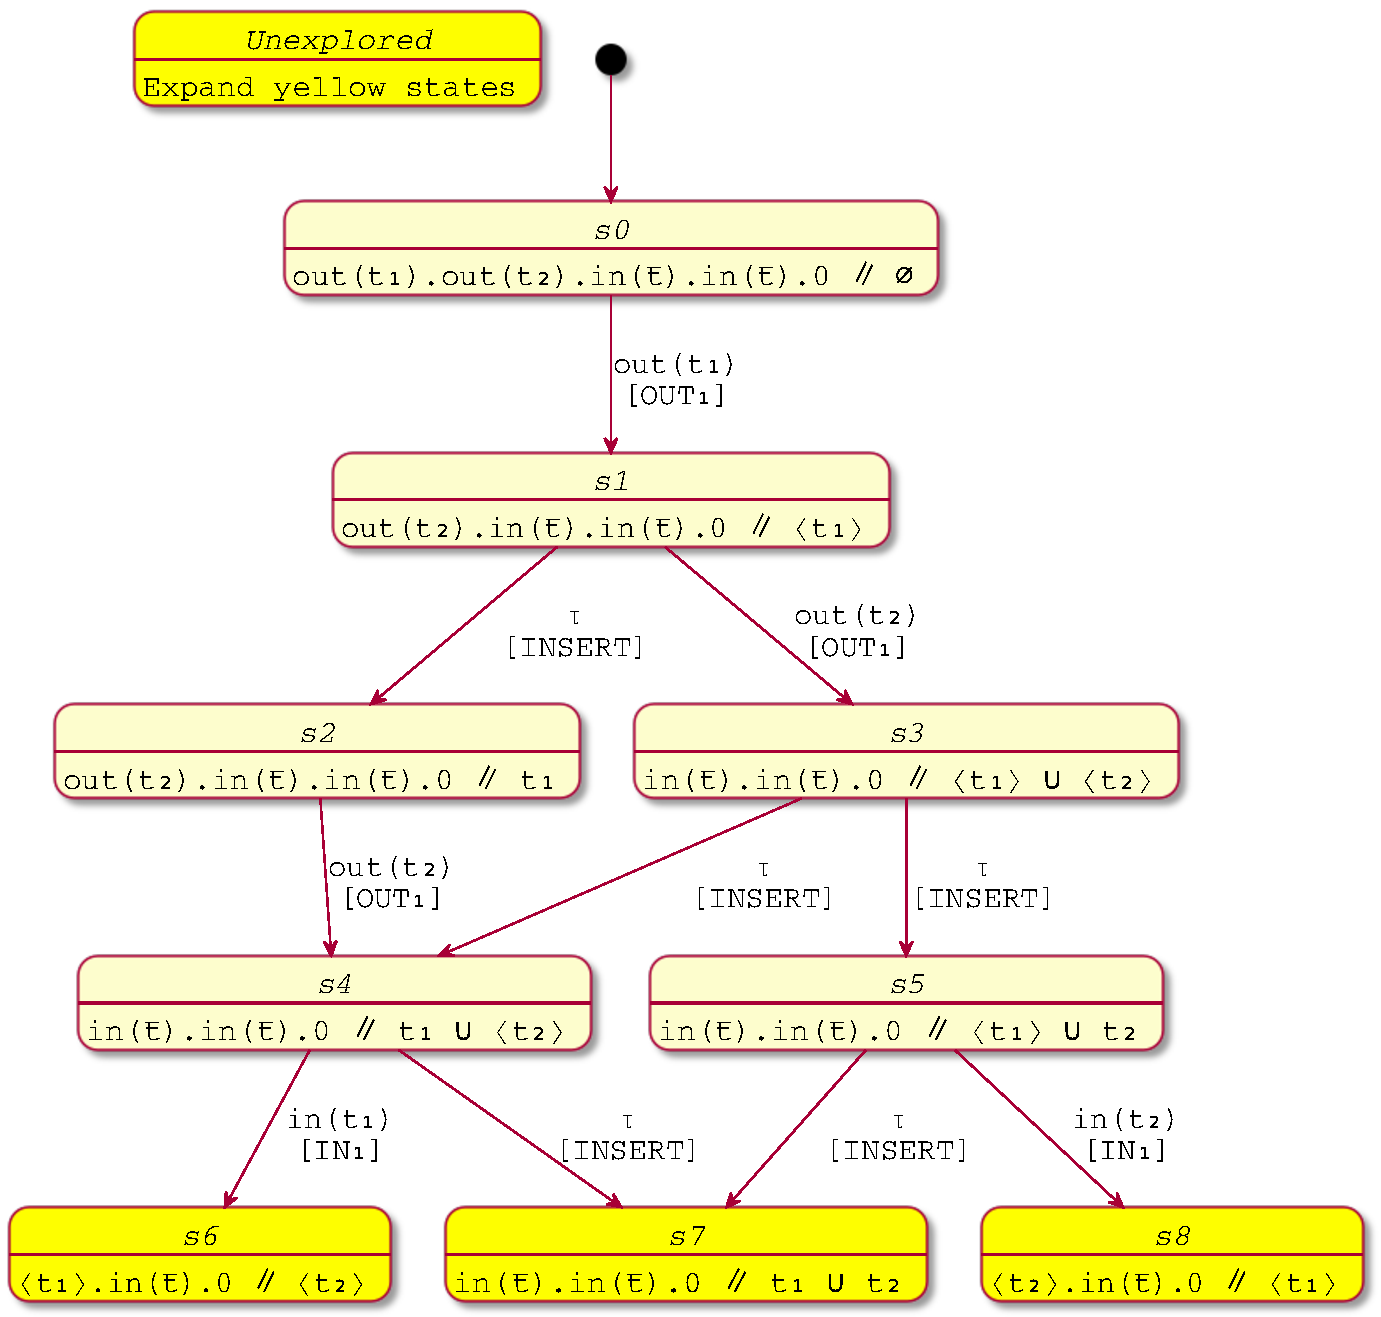
\includegraphics[width=.5\linewidth]{res/img/ex1.pdf}
    \end{center}
    \hint{Zoomable image \href{http://www.plantuml.com/plantuml/svg/ZPBFpj905CNtynHt-Nqca5B-G1f2Y8Y96qm4LiXYGaUSC9rfEbC5ZGiRJ5pm6YxaMKny1vx4ARULMejrGRYzTyxld3kPiJOqCd4WYDvn6TA81l2ClQ6nCC-LD7F-WO7h58PpGmsxZin1CE262hxHrUeP3HXCL1nn5f6tt6V0Wj0Sm6Tw4_7GS2L9GQbJD7ma04_fPhUDL2pzYH8g6WwdqkToEng14lmTgpgnb6mVsehvzjI12Q7Uaq-48FCsX3zFUZ3TXrJwcG8ZQ49MJzRGQ8n0EqYmXGSgDW_cadn-R6PLyjZayi7yEDx-7RXy_MP_NuXsaD0g25_BrSlbmbRhB1cEwsYdxwdwSZeJtKAewy7FewMzcCsdhnRht_tsZLPbvaAzMsf5j8ky3lmRsBRpkj3syvnz9jSTsXcxj4FUxvRww8LPxaV-owM3j1wAyFOjyne_7_RlM7N_TwtKZUXkDItl3_88II52RjM3qjlr2XwLvhWUgljbTTqLOU9SFgWsHu_xht3Cf1y7uXS0}{here}}
\end{frame}

\section{Several possible semantics}

\begin{frame}
\frametitle{Ordered VS unordered semantics for \linda{}}

    \begin{itemize}
        \item<1-3> The tuple spaces semantics defined so far is known as the \alert{unordered} semantics of \linda{}
        %
        \begin{itemize}
            \item<2-> long story short: if $n$ tuples are orderly \texttt{out}'d by an agent, you cannot assume them to be inserted into the tuple space in the same order
            \item<3> agents cannot use tuple spaces as counters $\implies$ \alert{no Turing equivalence}
        \end{itemize}
        
        \vfill
        
        \item<4> The unordered semantics essentially states the \texttt{out} operation is \emph{asynchronous}
        
        \vfill
        
        \item<5> We will now provide an \alert{ordered} semantics where the \texttt{out} primitive is \emph{synchronous}, making the resulting coordinated systems Turing equivalent
    \end{itemize} 

\end{frame}

\subsection{Ordered semantics}

\begin{frame}
\frametitle{Ordered semantics for \linda{}}

    \begin{enumerate}
        \item<1> Imagine the syntax for tuple spaces was defined without a means for expressing pending tuples to be inserted:
        %
        \[\begin{array}{rcl}
            TS &::=& (T \cup TS) \mid \emptyset
        \end{array}\]
        
        \vfill
        
        \item<2> Then, imagine transition rule $[\text{INSERT}]$ was never defined, neither for $\mathcal{TS}$ nor for $\mathcal{CS}$
        
        \vfill
        
        \item<3> Then, imagine transition rule $[\text{SCHEDULE}]$ was defined in the following way for $\mathcal{TS}$:
        %
        \[\begin{array}{rcl}
            TS &\xrightarrow{?out(t)}_\mathcal{TS}& (TS \cup t)
        \end{array}\]
        
        \vfill
        
        \item<4> Finally, imagine transition rule $[\text{OUT}_i]$ was defined in the following way for $\mathcal{CS}$:
        %
        \[
            \frac{
                \mathtt{out}(t) \cdot U_i \xrightarrow{\highlightG{!out(t)}}_\mathcal{U} U_i 
                \qquad
                TS \xrightarrow{\highlightG{?out(t)}}_\mathcal{TS} TS \cup t 
            }{
                US \parallel \highlightR{\mathtt{out}(t) \cdot U_i} \parallel US' \parallel \highlightB{TS}
                \xrightarrow{\highlightG{out(t)}}_\mathcal{CS}
                US \parallel \highlightR{U_i} \parallel US' \parallel \highlightB{TS \cup t }
            }
        \]
    \end{enumerate}

\end{frame}

\subsection{Exercise 5.2}

\begin{frame}
\frametitle{Exercise 5-2: Out-Out-In-In, \emph{ordered} I}
    \begin{enumerate}
        \item Go on working on your local clone of the Lab-5 GitLab repository
        
        \vfill
        
        \item Consider the system with \alert{$s_0 = \mathtt{out}(t_1) \cdot \mathtt{out}(t_2) \cdot \mathtt{in}(\bar t) \cdot \mathtt{in}(\bar t) \cdot 0  \parallel \emptyset$}, where $t_1, t_2 \in \bar{t}$, s.t. the \alert{ordered} \linda{} semantics defined before
        
        \vfill
    
        \item Complete the state graph according to the transition ruled defined before and include the state graph image in your \alert{\texttt{README.md}} file
        %
        \begin{itemize}
            \item web editor here: \href{
                http://www.plantuml.com/plantuml/uml/XO_1IiD048RlynHpR8MMjCTIacBLenvgJxM79JlMePlTi3khHl5WKV15V1kVeazYQeH627XOzeV__pwOMH3b9HO6mfPjgRmgy8nkLJHouQmi-8bmdBJAXIYXdqegGyYY3EUXcxvK1U7SHS_auOur8HMbLAWfv9vBOMUXHOQ36fy1yLJbsurtqUgvCyvFf-TMizsaAJh3zzIrM5fwBEj4kbvLP8nxW1U0rSaQ1uCKGmADFYGJT55wij-zzeU_QTSVikt9rzlnJt3_yLc_TmX9OnYrm1kxkbfUrsaDZRUf_x4TK0YZHZS-xhjqO_nxqmIpB8CPMHqBymq0
            }{http://www.plantuml.com/plantuml/uml/XO...q0}
        \end{itemize}
        
        \vfill
        
        \item On the state graph, edges' labels should show both:
        %
        \begin{itemize}
            \item the event raised by the transition
            \item the transition rule justifying the edge
        \end{itemize}
        
        \vfill
        
        \item You can rely on the tools listed on slide \ref{useful-tools} for your exercise
        
        \vfill
        
        \item Commit \& push your \texttt{README.md} file
        
    \end{enumerate}
    
\end{frame}

\begin{frame}
\frametitle{Exercise 5-2: Out-Out-In-In, \emph{ordered} II}

    \begin{center}
        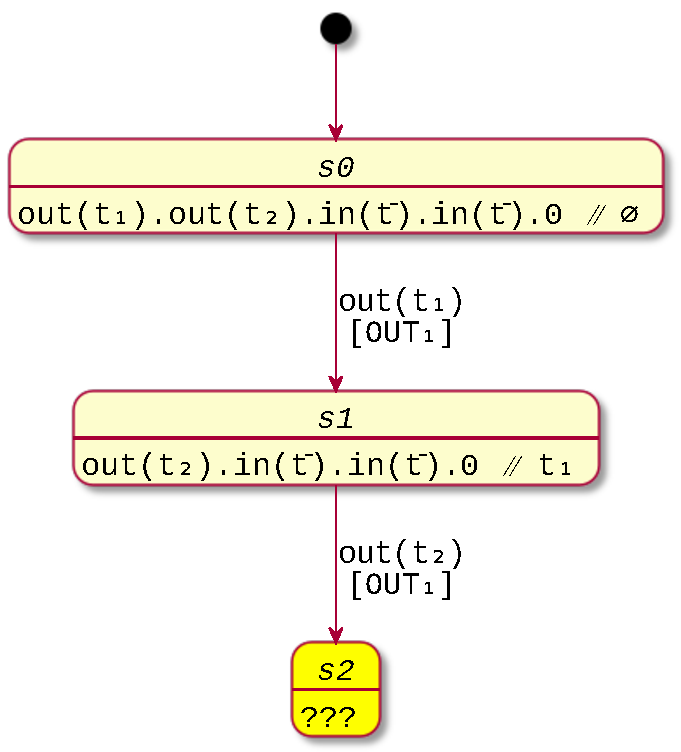
\includegraphics[width=.5\linewidth]{res/img/out-out-in-in.pdf}
    \end{center}

\end{frame}

\subsection{Exercise 5.3}

\begin{frame}
\frametitle{Exercise 5-3: Choice, \emph{ordered} I}
    \begin{enumerate}
        \item Go on working on your local clone of the Lab-5 GitLab repository
        
        \vfill
        
        \item Consider the system with \alert{$s_0 = (\mathtt{out}(t_1) + \mathtt{out}(t_2)) \cdot \mathtt{rd}(\bar{t}_3) \cdot 0 \parallel \mathtt{in}(\bar{t}_4) \cdot 0 \parallel (\mathtt{in}(\bar{t}_2) \cdot \mathtt{out}(t_3) + \mathtt{in}(\bar{t}_1) \cdot \mathtt{out}(t_4)) \cdot 0  \parallel \emptyset$}, where $t_i \in \bar{t}_i$ for all $i = 1,\ldots,4$, s.t. the \alert{ordered} \linda{} semantics defined before
        
        \vfill
    
        \item Complete the state graph according to the transition ruled defined before and include the state graph image in your \alert{\texttt{README.md}} file
        %
        \begin{itemize}
            \item web editor here: \href{
                http://www.plantuml.com/plantuml/uml/lO_1JW8n48RlVOeviXB8mf4GGbmnUj43yOGS6ZfYGxVTj5CLZGSg9ho8R-DJx9EuiDeWuQgtQV_ld_-VeIDkoUUAkONK1RSyXpEyurxHkT4qbiy8tNHF71Cdt4cqL0YIk98pTznznNE4p7WhqR9xAH0mBsW90jtCoeAaqMpFwRQh0LuOm2cVBURMU2qoeupjzqTQI3qV3C0e-O37Y1kDJqKreQYe9Ifb7jahOvEJARHQ0t0fs-slXXuqZAS6bM6LG1E-vv0aRIiQzBakmrlIJg7SV83KzSVwy2CaxTfNiyqehA8GFUNcdRcqRj7fGSo-rPFiuleo6rMFQIIwaGW7nCy17VXzRG_-flUsP0pj_bzeO4FKmkVg2m00
            }{http://www.plantuml.com/plantuml/uml/lO...m00}
        \end{itemize}
        
        \vfill
        
        \item On the state graph, edges' labels should show both:
        %
        \begin{itemize}
            \item the event raised by the transition
            \item the transition rule justifying the edge
        \end{itemize}
        
        \vfill
        
        \item You can rely on the tools listed on slide \ref{useful-tools} for your exercise
        
        \vfill
        
        \item Commit \& push your \texttt{README.md} file
        
    \end{enumerate}
    
\end{frame}

\begin{frame}
\frametitle{Exercise 5-3: Choice, \emph{ordered} II}

    \begin{center}
        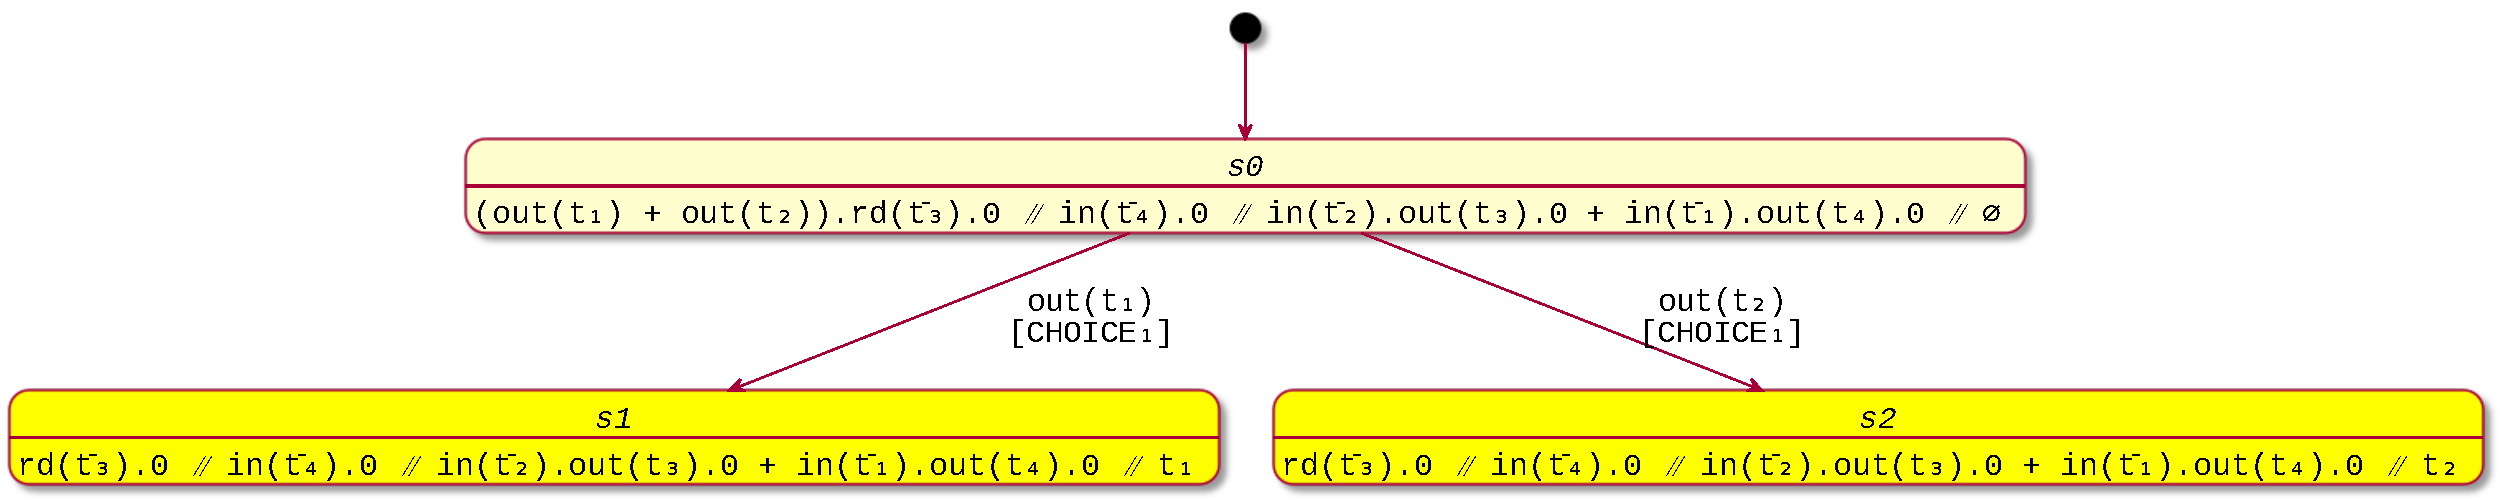
\includegraphics[width=\linewidth]{res/img/ex3.pdf}
    \end{center}
    
    \hint{Zoomable image \href{http://www.plantuml.com/plantuml/svg/lO_1JW8n48RlVOeviXB8mf4GGbmnUj43yOGS6ZfYGxVTj5CLZGSg9ho8R-DJx9EuiDeWuQgtQV_ld_-VeIDkoUUAkONK1RSyXpEyurxHkT4qbiy8tNHF71Cdt4cqL0YIk98pTznznNE4p7WhqR9xAH0mBsW90jtCoeAaqMpFwRQh0LuOm2cVBURMU2qoeupjzqTQI3qV3C0e-O37Y1kDJqKreQYe9Ifb7jahOvEJARHQ0t0fs-slXXuqZAS6bM6LG1E-vv0aRIiQzBakmrlIJg7SV83KzSVwy2CaxTfNiyqehA8GFUNcdRcqRj7fGSo-rPFiuleo6rMFQIIwaGW7nCy17VXzRG_-flUsP0pj_bzeO4FKmkVg2m00}{here}}

\end{frame}

\section*{}

\begin{frame}
\frametitle{Let's further simplify Users: abstracting $[\text{COMPUTE}]$ away}
    \begin{enumerate}
        \item<1> Imagine the syntax for users was simply defined as follows:
        %
        \[\begin{array}{rcl}
            U &::=& \mathtt{out}(T) \cdot U \mid \mathtt{in}(TT) \cdot U \\
            &\mid& \mathtt{rd}(TT) \cdot U \mid (U + U) \mid 0
        \end{array}\]
        
        \vfill
        
        \item<2> Then, imagine transition rule $[\text{COMPUTE}]$ and $[\text{COMPUTE}_i]$ where never defined, neither for $\mathcal{TS}$ nor for $\mathcal{CS}$
        
        \vfill
        
        \item<3> Then, imagine rule $[\text{IN}_i]$ was defined in the following way for $\mathcal{CS}$:
        %
        \[
    		\frac{
    			\mathtt{in}(\bar t) \cdot U_i \xrightarrow{\highlightG{?in(\bar t)}}_\mathcal{U} U_i 
    			\qquad
    			TS \cup t \xrightarrow{\highlightG{!in(t)}}_\mathcal{TS} TS
    			\qquad
    			t \in \bar{t}
    		}{
    			US \parallel \highlightR{\mathtt{in}(\bar t) \cdot U_i} \parallel US' \parallel \highlightB{TS \cup t}
    			\xrightarrow{\highlightG{in(t)}}_\mathcal{CS}
    			US \parallel \highlightR{U_i} \parallel US' \parallel \highlightB{TS}
    		}
    	\]
        
        \vfill
        
        \item<4> Finally, imagine rule $[\text{RD}_i]$ was defined in the following way for $\mathcal{CS}$:
        %
        \[
    		\frac{
    			\mathtt{rd}(\bar t) \cdot U_i \xrightarrow{\highlightG{?rd(\bar t)}}_\mathcal{U} U_i 
    			\qquad
    			TS \cup t \xrightarrow{\highlightG{!rd(t)}}_\mathcal{TS} TS \cup t
    			\qquad
    			t \in \bar{t}
    		}{
    			US \parallel \highlightR{\mathtt{rd}(\bar t) \cdot U_i} \parallel US' \parallel \highlightB{TS \cup t}
    			\xrightarrow{\highlightG{rd(t)}}_\mathcal{CS}
    			US \parallel \highlightR{U_i} \parallel US' \parallel \highlightB{TS \cup t}
    		} 
    	\]
    \end{enumerate}
\end{frame}

\subsection{Dining Philosophers}

\begin{frame}
\frametitle{Dining Philosophers}
    \columnsHH{
        \begin{itemize}
            \item<1> $N$ philosophers are sitting on a round table spending their time \alert{eating} and \alert{thinking} 
            
            \item<2> $N$ forks are on the table: philosopher $i$ has fork $i$ on his left and form $(i + 1) \% N$ on his right
            
            \item<3> In order to eat, philosopher $i$ must be holding \alert{both} fork $i$ and fork $(i + 1) \% N$
            
            \item<4> There is no way for a philosopher to take more than one fork \alert{at a time}
        \end{itemize}
    }{
        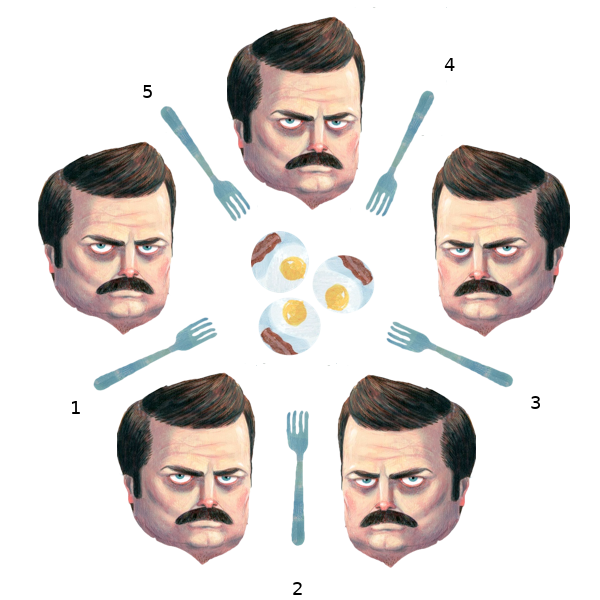
\includegraphics[width=\linewidth]{res/img/dining_pilosophers.png}
    }
\end{frame}

\subsubsection{Exercise 5.4}

\begin{frame}
\frametitle{Exercise 5-4: Three \href{https://en.wikipedia.org/wiki/Dining_philosophers_problem}{Dining Philosophers}, \emph{ordered} I}
    \begin{enumerate}
        \item Go on working on your local clone of the Lab-5 GitLab repository
        
        \vfill
        
        \item Consider the system with \alert{$\mathtt{in}(\bar{t}_1) \cdot \mathtt{in}(\bar{t}_2) \cdot \mathtt{out}(t_1) \cdot \mathtt{out}(t_2) \cdot 0 \parallel \mathtt{in}(\bar{t}_2) \cdot \mathtt{in}(\bar{t}_3) \cdot \mathtt{out}(t_2) \cdot \mathtt{out}(t_3) \cdot 0 \parallel \mathtt{in}(\bar{t}_3) \cdot \mathtt{in}(\bar{t}_1) \cdot \mathtt{out}(t_3) \cdot \mathtt{out}(t_1) \cdot 0 \parallel t_1 \cup t_2 \cup t_3$}, where $t_i \in \bar{t}_i$ for all $i = 1,\ldots,3$, s.t. the \alert{ordered} \linda{} semantics defined before
        
        \vfill
    
        \item Complete the state graph according to the transition ruled defined before and include the state graph image in your \alert{\texttt{README.md}} file
        %
        \begin{itemize}
            \item web editor here: \href{
                http://www.plantuml.com/plantuml/uml/R8-nJiCm441tVyMDBLAhq15L4Q85YQLBnTHsiEAZM77ioBu00J4qOU17MFWMlg9VWXDgPAHiJtVlMRvBHznILIZcSgbBRda1IxpdbQ8ResajNn1cIRHS4oViLrGh14bSoSmDrojU82nCPILQzY050XObrI3GPLQM98rcKUcwf-6L0LpnBDzRKscnCChO-VnQ2wdtQGf6oKSSCfR8XJ9PxXsBOiYuq_XSUaBXdHgLCa_iZR7DsGucanHSmleFUBW0gKVq_Nvi3kDfm6OyDHMDo0y3TRDagm6E7vyGUG7RI0pKdfB_KHkYwFKeFuJeb7KZ3ryTD05QvfBVIyxx0_fkgpUtAm-xl-NifncpnuaO1g9mdrFu2F6_dOeRq4191otDtc0ZxasapDDujICB0ybEGVK4-kRDUxO9n2l4AuiUuWfnVPlWYpMBKUf6QuBTHmdjd301OfHCW9Xw9ZZpXtGS7mcOuFPHifG4YELkpYkBjMU2D-TNPBWNqyLJ7MRH1QXMp09KT_Exy056XCq8BJsWpGS2zo3RoPzVN_QneOVUWkDerO-VAn9t55CBjTlTXAaKP9KYceWxYwSLr29555DbVRlAn5sbNK5rSszNvNT7p767wtGfn2rVhr3TmX3eNREjUlJzCJvN9N8lpWKrI2g_3MPztR9uyKIfN2odNhkirRSmQubSlDvPBYmBhpbtuYN-quqv8g_2IbZsyy9_4HrRspHwS_lUNuoY5_lAd47cV5Hnjf-lniLuH_V0OnXqW4k6_-aRGJl3kAnnhO0hYeshYXFdPht6EQlPE2V03TyxXtq_QLpq-ZOCjD3tyByv1-CN5HzuBYdkRTQRkA8wSLKX7U3yBC2T-j3kVoATdZu-txTl_jy0
            }{http://www.plantuml.com/plantuml/uml/R8...jy0}
        \end{itemize}
        
        \vfill
        
        \item On the state graph, edges' labels should show both:
        %
        \begin{itemize}
            \item the event raised by the transition
            \item the transition rule justifying the edge
        \end{itemize}
        
        \vfill
        
        \item You can rely on the tools listed on slide \ref{useful-tools} for your exercise
        
        \vfill
        
        \item Commit \& push your \texttt{README.md} file
        
    \end{enumerate}
    
\end{frame}

\begin{frame}
\frametitle{Exercise 5-4: Three Dining Philosophers, \emph{ordered} II}
    
    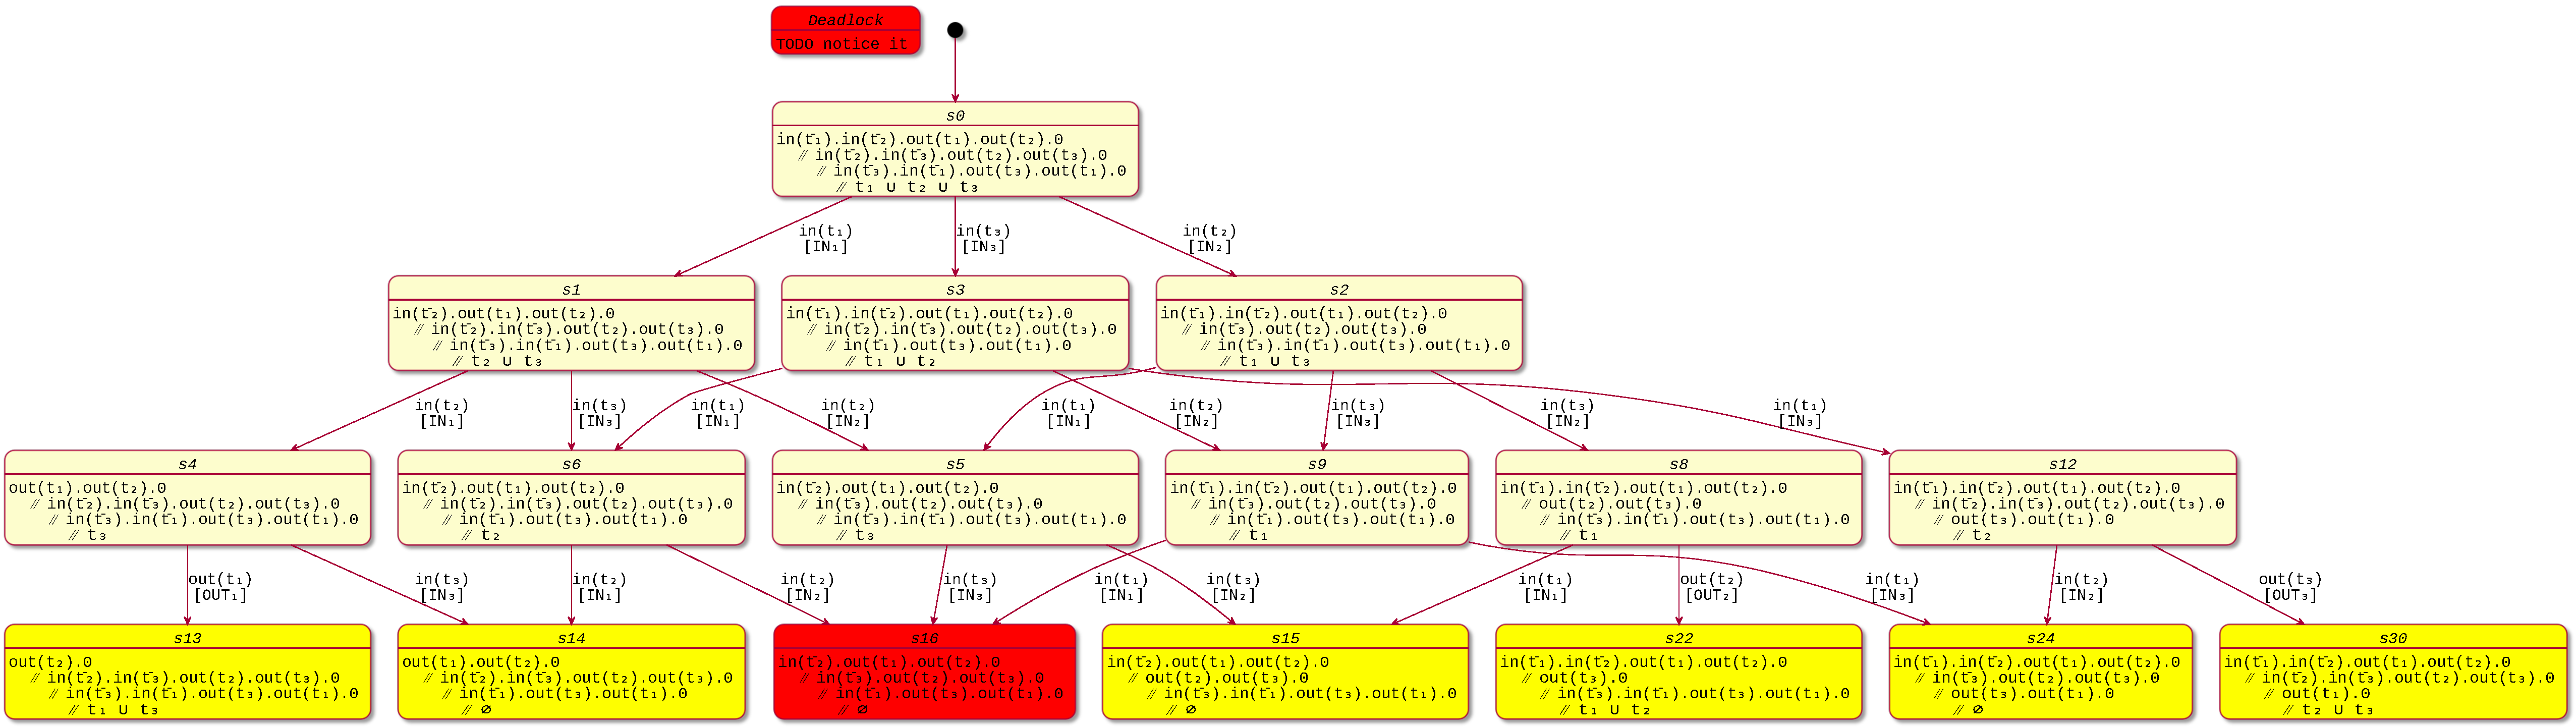
\includegraphics[width=\linewidth]{res/img/three_dining_philosophers.pdf}
    %
    \hint{SVG zoomable image available \href{http://www.plantuml.com/plantuml/svg/R8_1JW8n443l_OevWWbazKW8CO8cNk20di13inrnGhVTjBCg6W-21t_4Yz_YL_0bTgrDUjZRo_IzJkRSitJSL5huBPbQEbd13Ezbe_dA6bxI2y9PaJqkMJB-FV5E8n1BJQNlhkUoGfZQnX4wyK0A0QkQTw3Gbuvg9cj4LlhsQtWL01Uot6wSROoQMctTU7nf59dDP09MqoDs6JEKIjjo6no7gikuDVXS1q8Ld1rgRP_4cn1nQyeX_sa4DulP0enbAjjJXLYTtC5WC05Vn2x02CZq-EVZk7_l3nFk-qFRS8_3C54xAzO6uFZv1PcNy929YGx_IHP5CrkPr6nZYcBMZW9yjx1FS12-Y9USjWV4RcrMr_C0lyrNlMw6C0pSUOeymeVp8vAfRz2b7TdQjGjl0Efx5mbVJS6AcbQ134mdeRlpdJ7ZDqW0Pu2pW1RW0d0PE_ZIcsHQTEDWGhz9SQ9JJ03eDHC0Xfm9PFwHZlgHW0a4dKeI00uddRE0CMU2DPTNfBmNtMIv3YGkY1QWGRC8ODHo0XVSwa8h9U2nErPicHchUdvzsMG1Txdf-lAUrzRbcRTN8miqMzm0LGq4bVCPcBU-ge26N0Q7lpMntWxgfW6pqee5b2W92IHqfolMNhFbkYBceUa2IavGvGjA5oxENuQm9p1NSYQmVIHv8mQsbsRDptiicOQEf4LuEftdNQjWVJw5d3-HkwlH2hbmkAHlAgL2ZKZnhRXbrIvquNaCN-KbLsIYVUJ9rLzL-SF-wVtZRVsh_G80}{here}}
    
\end{frame}

\subsubsection{Deadlocks}

\begin{frame}
\frametitle{Deadlocks}
    \begin{block}{Deadlock}
        A situation where $N$ processes must access some shared resources in a mutually exclusive way and all of them get stuck, waiting for some other process to release a resource
    \end{block}
    
    \pause\vfill
    
    \vfill
    
    \begin{alertblock}{Deadlock on a state graph}
        Deadlocks are those states on a state graph having \alert{no outgoing edge}, i.e., those states where \alert{no transition rule} can be applied (red states on the image)
    \end{alertblock}

\end{frame}

\subsection{Formalising other primitives}

\begin{frame}
\frametitle{Formalising other primitives}
    
    \begin{enumerate}
        \item<1-> Imagine the syntax for users was extended as follows:
        %
        \[\begin{array}{rcl}
            U &::=& \mathtt{out}(T) \cdot U \\
            &\mid& \mathtt{in}(TT) \cdot U \\
            &\mid& \mathtt{rd}(TT) \cdot U \\
            &\mid& \alert{\mathtt{no}(TT) \cdot U} \\
            &\mid& \alert{\mathtt{inp}(TT)\ ?\ U : U} \\
            &\mid& \alert{\mathtt{rdp}(TT)\ ?\ U : U} \\
            &\mid& \alert{\mathtt{nop}(TT)\ ?\ U : U} \\
            &\mid& (U + U) \mid 0
        \end{array}\]
        
        \item<2> Subject to the following axioms:
        %
        \[\begin{array}{rcl}
            (X\ ?\ T : F) \cdot Y &\equiv& X\ ?\ (T \cdot Y) : (F \cdot Y)
        \end{array}\]
        
    \end{enumerate}
    
\end{frame}

\subsubsection{Exercise 5-5}

\begin{frame}
\frametitle{Exercise 5-5: Writing transition rules}

    \begin{enumerate}
    \item Go on working on your local clone of the Lab-5 GitLab repository
        
        \vfill
        
        \item Try extending the $\mathcal{CS}$ definition with new transition rules formally specifying the semantics of the \texttt{no}, \texttt{inp}, \texttt{rdp}, and \texttt{nop} primitives 
        
        \vfill
        
        \item You can rely on the tools listed on slide \ref{useful-tools} for your exercise
        
        \vfill
        
        \item Commit \& push your \texttt{README.md} file
        
    \end{enumerate}

\end{frame}

\begin{frame}
\frametitle{Exercise 5-5: Example for the \texttt{nop} primitive}

    For instance, the \texttt{nop} primitive could be defined by means of the following transition rules:
    %
    \[
		\frac{
			\forall t \in \bar{t} : TS \neq TS' \cup t
		}{
			US \parallel \highlightR{\mathtt{nop}(\bar t)\ ?\ U : U'} \parallel US' \parallel \highlightB{TS}
			\xrightarrow{\highlightG{nop(\bar t, \top)}}_\mathcal{CS}
			US \parallel \highlightR{U} \parallel US' \parallel \highlightB{TS}
		} 
		~[\text{NOP-T}_i]
	\]
	%
    \[
		\frac{
			\exists t \in \bar{t} : TS = TS' \cup t \quad 
		}{
			US \parallel \highlightR{\mathtt{nop}(\bar t)\ ?\ U : U'} \parallel US' \parallel \highlightB{TS}
			\xrightarrow{\highlightG{nop(\bar t, \bot)}}_\mathcal{CS}
			US \parallel \highlightR{U'} \parallel US' \parallel \highlightB{TS}
		} 
		[\text{NOP-F}_i]
	\]

\end{frame}

\section{Exercise 5-6: Coffee Machine}

\begin{frame}[allowframebreaks]
\frametitle{Exercise 5-6: Coffee Machine}
    
    \begin{enumerate}
        \item You must perform and end-to-end formalisation of a C/DS composed by a coffee machine and the user interacting with it
        
        \item The system must take into account the following requirements:
        %
        \begin{itemize}
            
            \item Any coffee machine simply performs the following sort of actions:
            %
            \begin{itemize}
                \item it initially \alert{waits} for \alert{coins} to be inserted
                \item it then \alert{checks} if coins are sufficient
                \item it may optionally give \alert{change} back to the user
                \item it serves the \alert{coffee} to the user
                \item it finally \alert{waits} for the \alert{user} to take the coffee 
            \end{itemize}
            
            \item In turn, any user can perform the following actions:
            %
            \begin{itemize}
                \item he/she can \alert{walk} around
                \item he/she can \alert{chat} with some friends
                \item he/she can insert coins into the coffee machine in order to \alert{pay}
                \item it can \alert{take} the coffee the machine has eventually served
            \end{itemize}
            
            \item Of course, coffee machines can stop waiting for money only if some user pays 
            %
            Similarly, they can stop waiting for the coffee to be taken only if some user takes it
        \end{itemize}
        
        \item Your formalisation must provide an interpretation and a semantics for the following formula:
        \\\vspace{.1cm}
        \alert{$
            s_0 = (\mathtt{chat} + \mathtt{walk}) \cdot \mathtt{insert} \cdot (\mathtt{walk} + \mathtt{chat}) \cdot \mathtt{take} \cdot 0
        $\\\hfill$    
            \quad\parallel
            \mathtt{waitCoin} \cdot \mathtt{check} \cdot (\mathtt{change} \cdot \mathtt{coffee} + \mathtt{coffee}) \cdot \mathtt{waitUser} \cdot 0
        $}
        
        \item Draw the state graph of the system having $s_0$ as initial state, according to your semantics
        
        \item You can rely on the tools listed on slide \ref{useful-tools} for your exercise
        
        \item Commit \& push your \texttt{README.md} file
        
    \end{enumerate}
    

\end{frame}

\section{Useful tools}

\begin{frame}\label{useful-tools}
\frametitle{Useful tools}
    
    \begin{itemize}
        \item Web-based markdown editor supporting \LaTeX{} syntax for formulas
        %
        \begin{itemize}
            \item \url{https://upmath.me}
        \end{itemize}
        
        \vfill
        
        \item Web-based \href{http://plantuml.com/}{PlantUML} editor for designing State Charts (and other UML diagrams)
        %
        \begin{itemize}
            \item \href{http://www.plantuml.com/plantuml/uml/XOz1JW8n58RtFSLRWWbaW1qXG4HCt60Yi48MpVI93Prsqhwget4XmSG5rt2XPp7n3dCI2uYEoIGkclxfz_wlUNr7t99F57DBgLDkUG8dUCMzebEZQIpl4PfH0Ow94-uGPGf14bSoTkNj4KyG1iPRYPPTIu60IKeP27InbIb9ercXwRPgU600npnUBgpnMWoCChRJ6MeXzQBR1QFa3PPDJ3NUfI6X25CPAcLksIDZiwCvr6fTS17RwKDeW_5KeNprLAr_frMrBdM5FjQ_TmJvosiupyn5UqEZKBpKi_Ff9AGvEtW3_jUsUTksyyqxSuszjDc6ptMmdOt6mul9_EUzLR2LVDQ4lnkteTVh7M2h5FPH2v-eBm00}{\texttt{http://plantuml.com/plantuml}}
        \end{itemize}
        
        \vfill
        
        \item Web-based tool for converting \LaTeX{} formulas into Unicode strings
        %
        \begin{itemize}
            \item \url{http://vikhyat.net/projects/latex_to_unicode}
        \end{itemize}
    \end{itemize}
    
\end{frame}

\maketitle

%%%%%%%%%%%%%%%%%%%%%%%%%%%%%%%%%%%%%%%%%%%%%%%%%%%%%%%%%%%%%%%%%%%%%%%%%%%%%%%
\end{document}
%%%%%%%%%%%%%%%%%%%%%%%%%%%%%%%%%%%%%%%%%%%%%%%%%%%%%%%%%%%%%%%%%%%%%%%%%%%%%%%%
